\documentclass[12pt,a4paper,ngerman]{report}
\usepackage{babel}
%\usepackage{natbib}
\usepackage{url}
%\usepackage[left=2cm, right=1.5cm, top=2cm, bottom=2cm]{geometry}
%\usepackage[ansinew]{inputenc}
\usepackage{amsmath}
\usepackage{nicefrac} % macht schöne Brüche mit querstrich mit \nicefrac{1}{2}
\usepackage{graphicx}
%\graphicspath{}
\usepackage{titlesec}% um chapterüberschriften anzupassen.
\titleformat{\chapter}{\normalfont\huge\bf}{\thechapter.}{20pt}{\huge\bf}
\usepackage{parskip}
\usepackage{fancyhdr}
\usepackage{amsfonts}
\usepackage{float}
\usepackage{caption}
\usepackage{subcaption} % for \begin{subfigure}
	
\usepackage{csquotes} % mit \enquote{blabla} tolle anfürungsstriche erstellen
%\usepackage{physics} %lässt mich \bra und \ket benuzen %im konflict mit siunitx

\usepackage{pgfplots} %für plots
\pgfplotsset{compat=newest}

\usepackage{varioref} % macht mit \vref{} viel bessere referenzen
\usepackage{hyperref} % macht klickbare referenzen

\usepackage{xcolor, soul} %mit \hl{} kann man toll Sachen hervorheben.
\newcommand{\highlight}[1]{%
	\colorbox{yellow!50}{$\displaystyle#1$}} % mit \highlight{} kann man sogar in Gleichungen hervorheben

\usepackage{vmargin}
\usepackage[section]{placeins}
\usepackage{capt-of}
\usepackage{enumitem}
\usepackage{multirow}
\usepackage{blindtext}
\usepackage[version=4]{mhchem} % um Chemische Elementsymbole zu benutzen: \ce{H20}

\usepackage{pdfpages} % um PDFs einzufügen

%spread to latex:
\usepackage{booktabs, multirow} % for borders and merged ranges
\usepackage{changepage,threeparttable} % for wide tables

\providecommand{\e}[1]{\ensuremath{\cdot 10^{#1}}}
\providecommand{\fehlt}{\textcolor{red}{\emph{Fehlt!\dots}}}

\usepackage{siunitx}
\sisetup{
	separate-uncertainty = true,
	%per-mode = fraction,
	%per-mode = symbol
}
\DeclareSIUnit\bar{bar}
\DeclareSIUnit\atomicmassunit{u}



\setmarginsrb{3 cm}{2.5 cm}{3 cm}{2.5 cm}{1 cm}{1.5 cm}{1 cm}{1.5 cm}
\title{UI-Kennlinien}			%%%%%%%%%%
% Title


\author{Frederik Uhlemann, F. Adamczyk}
% Author
\date{\today}
% Date

\makeatletter
\let\thetitle\@title
\let\theauthor\@author
\let\thedate\@date
\makeatother

\pagestyle{fancy}
\fancyhf{}
\rhead{\theauthor}
\lhead{UI-Kennlinien}
\cfoot{\thepage}
%%%%%%%%%%%%%%%%%%%%%%%%%%%%%%%%%%%%%%%%%%%%
\begin{document}
		
	%%%%%%%%%%%%%%%%%%%%%%%%%%%%%%%%%%%%%%%%%%%%%%%%%%%%%%%%%%%%%%%%%%%%%%%%%%%%%%%%%%%%%%%%%
	
	\begin{titlepage}
		\centering
		\vspace*{0.5 cm}
		% \begin{large} Justus-Liebig-Universität\\ Gießen \end{large}
		\includegraphics[width = 0.6 \textwidth]{JLU_Giessen-Logo}	%University Logo
		\\[2.0 cm]
		% \begin{center}    \textsc{\Large Justus - Liebig - Universität}\\{Giessen}\\[0.8cm]	\end{center}% University Name
		Versuch 4 des\\
		\textsc{\Large  Fortgeschrittenen-Praktikums}\\ [0.3 cm]				% Course Code
		\rule{\linewidth}{0.2 mm} \\[0.4 cm]
		{ \huge \bfseries \thetitle}\\%%% TITEL HERE
		\rule{\linewidth}{0.2 mm}\\
		Versuchstermin Freitag, 17.05.2024 \\
		~ \\
		[2.0 cm]
		
		
		\begin{minipage}{0.49\textwidth}
			\begin{flushleft}
				\emph{Praktikumsbetreuer:}\\
				Marius Müller\\
				%  Affiliation\\
				\small{\href{mailto:marius.mueller@physik.uni-giessen.de}{marius.mueller@physik.uni-giessen.de}}
			\end{flushleft}
		\end{minipage}~
		\begin{minipage}{0.49\textwidth}
			\begin{flushright}
				\emph{Protokoll von:} \\
				
				\large{Frederik Uhlemann}\\
				\small{\href{mailto:frederik-vincent.uhlemann@physik.uni-giessen.de}{frederik-vincent.uhlemann@physik.uni-giessen.de}\\~\\
					%Matrikel Nr.: \:  \\[0.5cm]
					%\href{mailto:}{}
				}
				\large{Florian Adamczyk} \\
				\small{\href{mailto:florian.marius.adamczyk@physik.uni-giessen.de}{florian.marius.adamczyk@physik.uni-giessen.de}\\
					%Matrikel Nr.: \: 8105234}
			}
		\end{flushright}
	\end{minipage}
	
	\end{titlepage}
	
%%%%%%%%%%%%%%%%%%%%%%%%%%%%%%%%%%%%%%%%%%%%%%%%%%%%%%%%%%%%%%%%%%%%%%%%%%%%%%%%%%%%%%%%%
\setcounter{secnumdepth}{3}
\setcounter{tocdepth}{4}
\tableofcontents
%\newpage

%%%%%%%%%%%%%%%%%%%%%%%%%%%%%%%%%%%%%%%%%%%%%%%%%%%%%%%%%%%%%%%%%%%%%%%%%%%%%%%%%%%%%%%%%
%\renewcommand{\thesection}{\arabic{section}} %lässt in den subsections die erste zahl von darüberliegenden chapter weg.

%\pagebreak
	
%\setcounter{chapter}{-1}
\chapter*{Einleitung}
	\addcontentsline{toc}{chapter}{Einleitung}
	\fehlt



\chapter{Versuchsaufbau und Durchführung}
	\fehlt

\chapter{Auswertung}
	\fehlt

	\section{Diode}
	
	\section{Bipolartransistor}
		\begin{figure}[h]
			\centering
			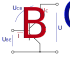
\includegraphics[width=7.5 cm]{plots/transistor_schaltung.png}
			\caption{Schaltskizze eines pnp-Transistors}
			\label{img:pnpSchaltung}
		\end{figure} 
		Im folgendem Versuchsteil werden die typischen Kennlinienfelder eines Bipolartransistors vermessen. Es handelt sich um einen pnp-Transistor des Typs BC550. Ein Schaltplan solch eines Transistors ist in Abbildung \ref{img:pnpSchaltung} dargestellt. Dabei sind die wichtigsten Größen eingetragen, dazu zählen der Kollektor- und Basisstrom $I_C$ und $I_B$, zudem die jeweiligen Spannungen zwischen Kollektor, Emitter und Basis. 
		\subsection{Vierpolarparameter}
				\begin{figure}[h]
			\centering
			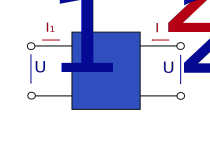
\includegraphics[width=7.5 cm]{plots/Vierpol.pdf}
			\caption{allgemeiner Vierpol}
			\label{img:Vierpol}
		\end{figure} 
		Jedes elektronische Bauteil kann als Vierpol dargestellt werden, in Abbildung \ref{img:Vierpol} ist der Schaltplan eines allgemeinen Vierpols angegeben. Das Modell beschreibt ein elektrisches Netzwerk oder Bauteil durch zwei Ein- und Ausgänge, dabei wird eine lineares Gleichungssystem mit einer 2x2 Matrix verwendet.\\
		Transistoren sind aktive Bauelemente und nicht linear, deshalb müssen sie in einem Punkt linearisiert werden, damit die Beschreibung des Vierpols angewandt werden kann. Dieser Punkt heißt Arbeitspunkt des Transistors. Für Transistoren in der Emittersschaltung wird häufig die folgende Hybrid-Darstellung verwendet:
		\begin{equation}
			\begin{pmatrix}
				u_{BE}\\
				i_C
			\end{pmatrix}
		=	\begin{pmatrix}
				h_{11} & h_{12}\\
				h_{21} & h_{22}\\
			\end{pmatrix}
		=	\begin{pmatrix}
				i_{B}\\
				u_{CE}
			\end{pmatrix}
		\end{equation}
		Wie bereits erwähnt wird am Arbeitspunkt des Transistors linearisiert, deshalb sind die Vierpolparameter Ableitungen in der folgenden Form:
		\begin{equation}
			\begin{split}
				h_{11} = \frac{\partial U_{BE}}{\partial I_{B}} \qquad h_{12} = \frac{\partial U_{BE}}{\partial U_{CE}}\\
				h_{21} = \frac{\partial I_{C}}{\partial I_{B}} \qquad h_{22} = \frac{\partial I_{C}}{\partial U_{CE}}\\
			\end{split}
		\end{equation}
		\subsection{Bestimmung der Parameter}
	\begin{figure}[h]
			\centering
			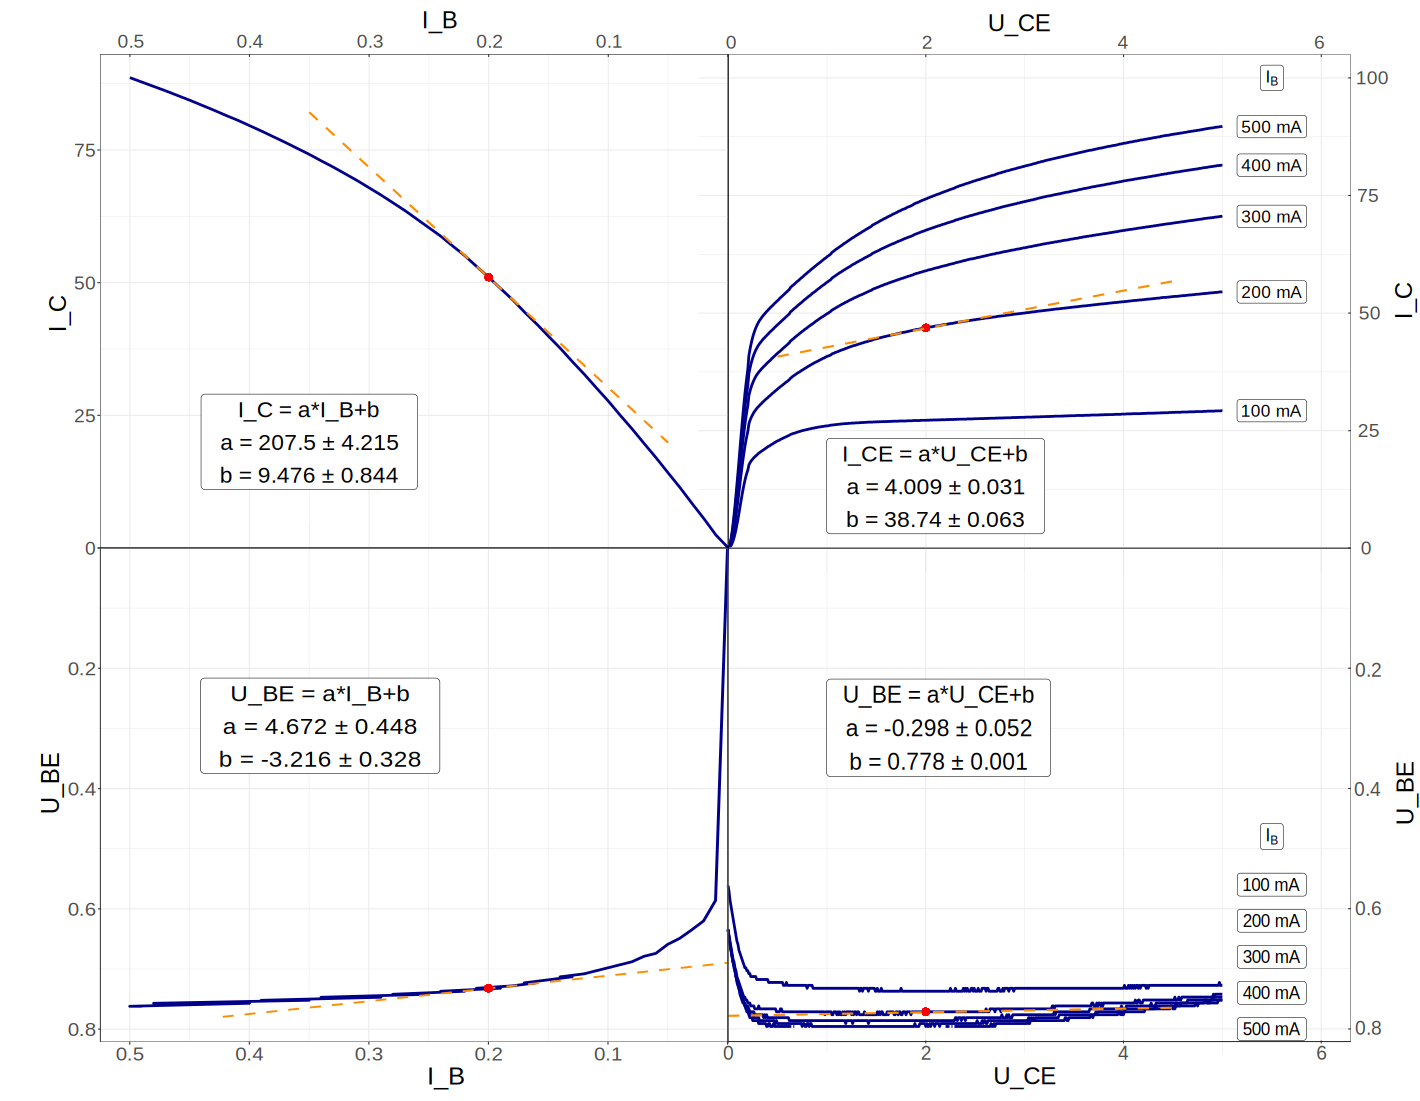
\includegraphics[width=\textwidth]{plots/Vierquadrantenkennlinienfeld.pdf}
			\caption{Vierquadrantenkennlinienfeld des Bipolartransistors}
			\label{img:Vierquadranten}
	\end{figure}
	In Abbildung \ref{img:Vierquadranten} sind die aufgenommen, typischen vier Kennlinien des Transistors aufgetragen. In Rot ist jeweils der gewählte Arbeitspunkt eingetragen, dieser wird folgenden Werten gewählt:
	\begin{equation}
		I_B = \SI{0.2}{\milli \ampere} \qquad U_{CE} = \SI{2}{\volt}
	\end{equation}
	Zudem in orange ist die jeweilige Fitgerade eingezeichnet und die Fitparameter sind gegeben.\\
	Der erste Vierpolparameter ergibt sich aus der Eingangskennlinien, also der $U_{BE}$-$I_B$-Kennlinie. Dieser Parameter ist direkt der differentielle Transistor-Eingangswiederstand:
	\begin{equation}
		r_{BE} = \frac{\Delta U_{BE}}{\Delta I_{B}}
	\end{equation}
	Im obigen Kennlinienfeld wurde die Gerade in einem Bereich von \SI{0.05}{\milli \ampere} um den Arbeitspunkt für $I_B$ zu $U_{BE}$ gefittet. Der differentielle Eingangswiederstand ist damit der Kehrwert des Fitparameters $a$, zudem werden die \si{\milli \ampere} in \si{\ampere} umgerechnet, um die Einheit \si{\ohm} zu erhalten:
	\begin{equation}
		r_{BE} = \frac{1}{a} = \underline{\SI{214.041(20.525)}{\ohm} = h_{11}}
	\end{equation}
	Der Vierpolparamter $h_22$ kann im Ausgangskennlinienfeld über den differentiellen Transistor-Ausgangswiderstand bestimmt werden. Der Widerstand ist die Steigung des Fits, erneut werden die \si{\milli \ampere} in \si{\ampere} umgerechnet:
	\begin{equation}
		r_{CE} =  \frac{\Delta U_{CE}}{\Delta I_{C}} = \SI{4009(31)}{\ohm}
	\end{equation}
	Der dazugehörige Vierpolparameter berechnet sich aus dem Kehrwert des Ausgangswiderstands:
	\begin{equation}
		\underline{h_{22} = \SI{2.494(19)E-4}{1 \per \ohm}}
	\end{equation}
	Aus dem Stromsteuerungskennlinienfeld $I_C$-$I_B$ kann der differentielle Stromverstärkungsfaktor $\beta$ bestimmt werden. Dieser ist entspricht dem Anstieg der gefitten Geraden und gibt in gewisser Weise an, um welchen Faktor der Transistor den Kollektorstrom verstärkt. Dieser Faktor ist auch der Vierpolparameter $h_{21}$:
	\begin{equation}
		\beta =  \frac{\Delta I_{C}}{\Delta I_{B}} = \underline{207.5 \pm 4.2 = h_{21}}
	\end{equation}
	Der letzte Vierpolparameter ist im Rückwirkungskennlinienfeld der differentielle Rückwirkungsfaktor $D$. Dieser gibt an wie stark Änderungen der Ausgangsspannung $U_{CE}$ auf die Eingangsspannung $U_BE$ zurückwirken. Solche sind unerwünscht un sollen möglichst klein sein. 
	\begin{equation}
		 D = \frac{\Delta U_{BE}}{\Delta U_{CE}} = \underline{-0.298 \pm 0.052 = h_{12}}
	\end{equation}
	\section{Solarzelle}



\chapter{Fazit}

	\listoffigures
	\addcontentsline{toc}{chapter}{\listfigurename}
	
	\begin{thebibliography}{111} \addcontentsline{toc}{chapter}{Literaturverzeichnis}
		\bibitem{Anleitung}
		I. Physikalisches Institut, \glqq Versuch 1.8: I-U-Kennlinien an Halbleitern
		und Solarzellen \grqq{}, 2024.
		
		\bibitem{beuth}
		K. Beuth, \glqq Elektronik 2 – Bauelemente\grqq, Vogel Buchverlag (Bauelemente)
		
		\bibitem{hunklinger}
		S. Hunklinger, \glqq Festkörperphysik\grqq, Oldenbourg Wissenschaftsverlag (Grundlagen)
		
		
		
	\end{thebibliography}


\chapter*{Anhang} \label{ch:Anhang}
\addcontentsline{toc}{chapter}{Anhang}
\FloatBarrier





\end{document}
